% Metody inzinierskej prace
\documentclass[10pt,twocolumn,twoside,slovak,a4paper]{article}

\usepackage[slovak]{babel}
\usepackage[IL2]{fontenc} 
\usepackage[utf8]{inputenc}
\usepackage{graphicx}
\usepackage{url} 
\usepackage{hyperref} 
\usepackage{cite}

% Pridané balíčky pre úlohy 3.6 a 3.7
\usepackage{multirow}
\usepackage[table]{xcolor}
\usepackage{amsmath}

\pagestyle{headings}

\title{Názov\thanks{Semestrálny projekt v predmete Metódy inžinierskej práce, ak. rok 2026/27, vedenie: Afanasiev Maksym}}

\author{Afanasiev Maksym\\[2pt]
	{\small Slovenská technická univerzita v Bratislave}\\
	{\small Fakulta informatiky a informačných technológií}\\
	{\small \texttt{...@stuba.sk}}
	}

\date{\small 13. október 2026}

% Úloha 3.5: Vlastné počítadlo
\newcounter{polozky}
\newcommand{\Polozka}{
  \refstepcounter{polozky}
  Položka číslo \thepolozky:
}

\begin{document}

\maketitle

\begin{abstract}
\ldots
\end{abstract}

\section{Úvod}
Motivujte čitateľa a vysvetlite, o čom píšete. Úvod sa väčšinou nedelí na časti.

Uveďte explicitne štruktúru článku. Tu je nejaký príklad.
Základný problém, ktorý bol naznačený v úvode, je podrobnejšie vysvetlený v časti~\ref{nejaka}.
Dôležité súvislosti sú uvedené v častiach~\ref{dolezita} a~\ref{dolezitejsia}.
Záverečné poznámky prináša časť~\ref{zaver}.

\section{Nejaká časť} \label{nejaka}
Z obr.~\ref{f:rozhod} je všetko jasné. 

\begin{figure*}[tbh]
\centering
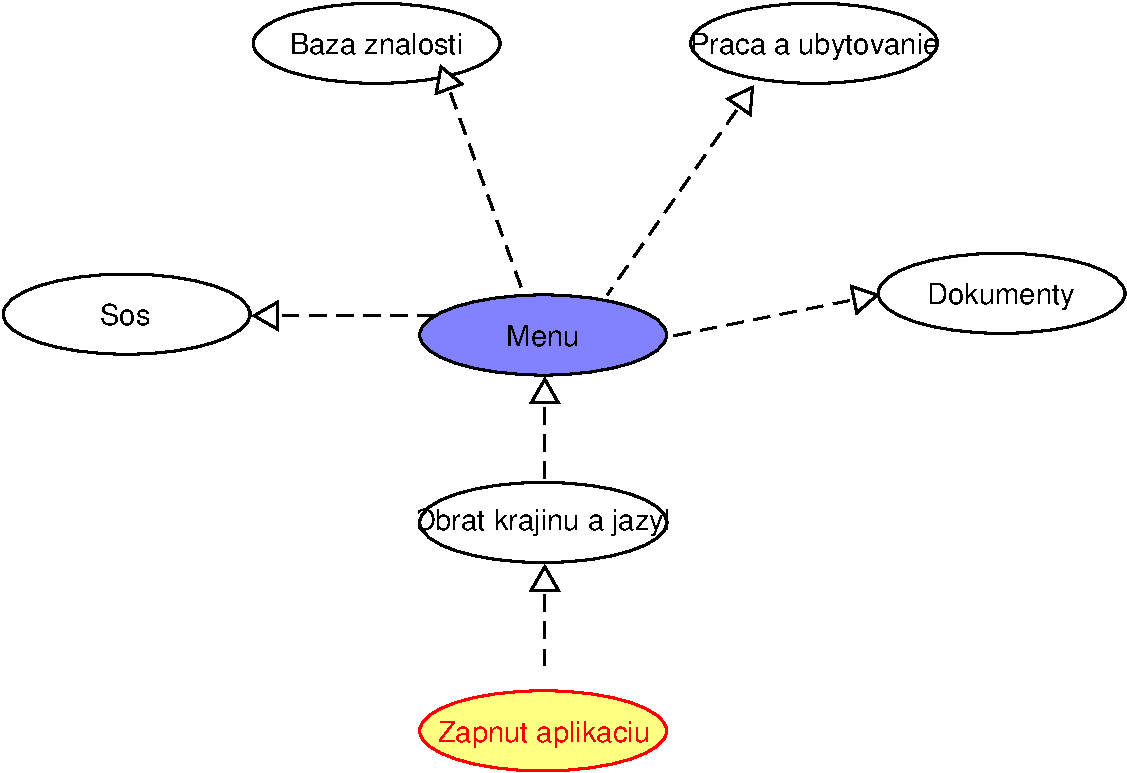
\includegraphics[width=\textwidth]{diagram-crop.pdf}
Aj text môže byť prezentovaný ako obrázok. Stane sa z neho označný plávajúci objekt. Po vytvorení diagramu zrušte znak \texttt{\%} pred príkazom \verb|\includegraphics| označte tento riadok ako komentár (tiež pomocou znaku \texttt{\%}).
\caption{Rozhodujúci argument.}
\label{f:rozhod}
\end{figure*}

\section{Iná časť} \label{ina}

% Umiestnenie testu vlastného počítadla
\Polozka{} Toto je prvý test vlastného príkazu. \\
\Polozka{} Toto je druhý test.

Základným problémom je teda\ldots{} Najprv sa pozrieme na nejaké vysvetlenie (časť~\ref{ina:nejake}), a potom na ešte nejaké (časť~\ref{ina:nejake}).\footnote{Niekedy môžete potrebovať aj poznámku pod čiarou.}

Môže sa zdať, že problém vlastne nejestvuje\cite{Coplien:MPD}, ale bolo dokázané, že to tak nie je~\cite{Czarnecki:Staged, Czarnecki:Progress}. Napriek tomu, aj dnes na webe narazíme na všelijaké pochybné názory\cite{PLP-Framework}. Dôležité veci možno \emph{zdôrazniť kurzívou}.

\subsection{Nejaké vysvetlenie} \label{ina:nejake}
Niekedy treba uviesť zoznam:

\begin{itemize}
\item jedna vec
\item druhá vec
	\begin{itemize}
	\item x
	\item y
	\end{itemize}
\end{itemize}

% Úloha 3.6: Zložitá tabuľka
\begin{table}[h]
\centering
\begin{tabular}{|l|c|c|}
\hline
\rowcolor{yellow} \multicolumn{3}{|c|}{\textbf{1. semester - povinné predmety}} \\
\hline
\textbf{Predmet} & \textbf{Suma udalostí} & \textbf{Kredity} \\
\hline
Metódy inžinierskej práce & \itshape{2000} & 4 \\
\hline
\multirow{2}{*}{Algebra a diskrétna matematika} & 4000 & \cellcolor{pink} 6 \\
 & 5000 & 6 \\
\hline
\end{tabular}
\caption{Ukážka formátovanej tabuľky}
\end{table}

\subsection{Ešte nejaké vysvetlenie} \label{ina:este}
\paragraph{Veľmi dôležitá poznámka.}
Niekedy je potrebné nadpisom označiť odsek. Text pokračuje hneď za nadpisom.

\section{Dôležitá časť} \label{dolezita}

% Úloha 3.7: Matematika
Ukážka zarovnania rovníc pod sebou:
\begin{align}
-3a &= 2b - 13 \\
4b + 3a - 5 &= 21 \\
D &= b^2 - 4ac \nonumber
\end{align}

\section{Ešte dôležitejšia časť} \label{dolezitejsia}

% Úloha 3.8: Logá
Tento dokument bol vytvorený pomocou systému \LaTeXe, ktorý stavia na základoch \TeX{} a využíva Bib\TeX{} pre správu literatúry.

\section{Záver} \label{zaver} 

\bibliography{literatura}
\bibliographystyle{plain} 
\end{document}